\section*{Validation}
\addcontentsline{toc}{section}{Validation}

The validation of the prototype was conducted with the help of seven user interviews. As mentioned by Butz and Krüger \cite{ButzKrueger2017} seven evaluators discover most part of the problems (around 80 percent). User interviews are a valid method to evaluate a prototype. They were conducted according to the usability test method of "think out loud", as mentioned in the \ac{MMST}-lecture. Each interviewee saw the finished prototype for the first time. They were required to think out loud about what is displayed on screen and what the different elements resemble. In addition to just looking at the screen, the interviewee was also asked to interact with the system. The users were ages 22 through 26. Six of them were college students and one interviewee was a master craftsman. They had no known background information about industrial furnaces. In the following, the major elements are discussed in their success and purpose based on the information gathered throughout the interviews. 

\begin{figure*}[htp]
    \centering
    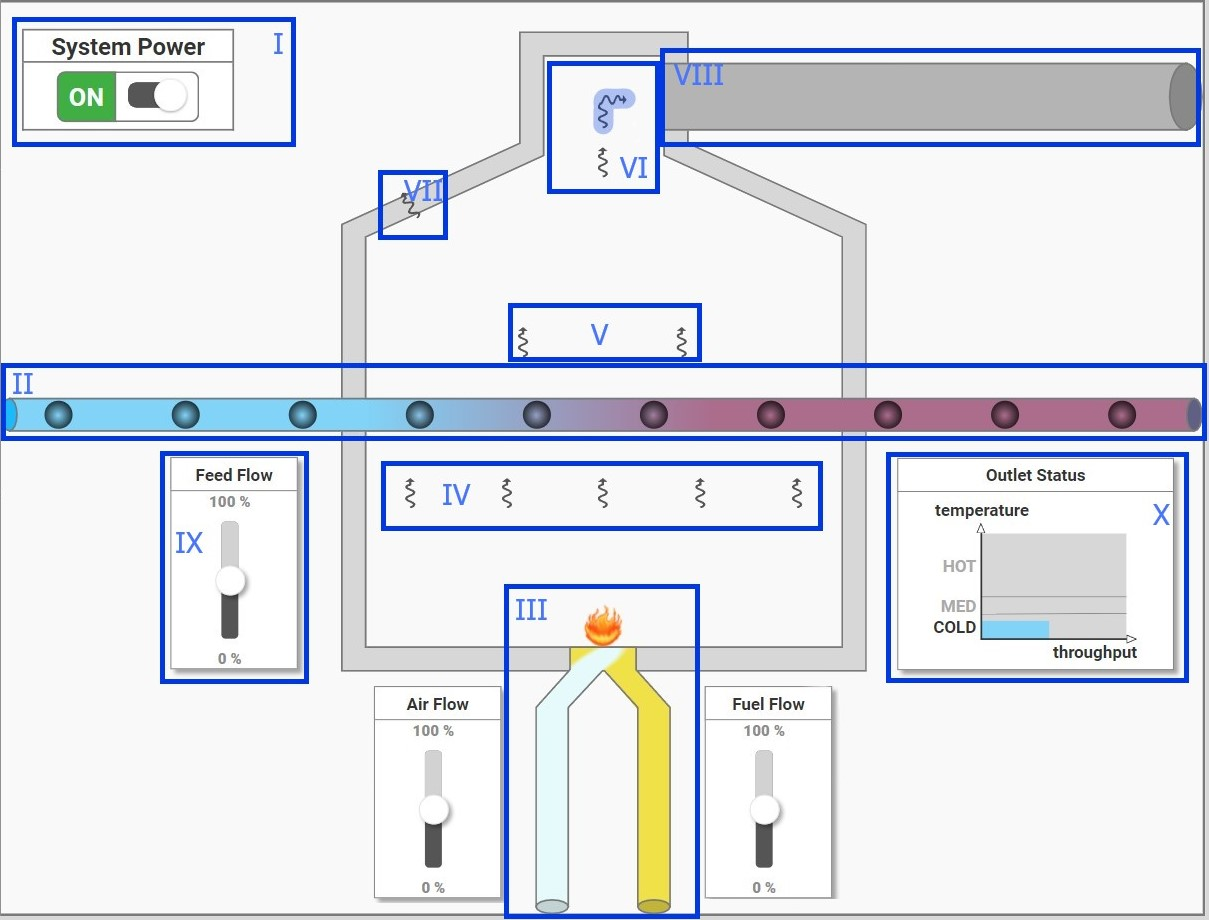
\includegraphics[width=0.7\linewidth]{images/concept/prototype/prototype_final_ref.jpg}
    \caption{prototype with highlights}
\label{fig:final_prototype_ref}
\end{figure*}

The ON/OFF switch (figure \ref{fig:final_prototype_ref} I) was changed because of some interviews, where users could not accurately say, what state the button is in. An ON/OFF sign was added next to it to further clarify that. This change however resulted in another problem. Now some users tried to click on the sign instead of the button. In a new approach this is something to look into and maybe exchange the switch completely and make the ON/OFF sign interactable for better clarity.

The heating process of the feed was always clear to understand because of the fade in color. The red end of the pipe (figure \ref{fig:final_prototype_ref} II) was correctly interpreted as the heated feed. Changing flow rate and therefore the resulting heat of the outlet was always intuitive. However, the blue color of the pipe and the "bubbles" moving through it produced the misunderstanding of the feed being water. It should have been undefined and could cause trouble in an approach where the feed is defined to not be water. In this case, the characterisation of coldness demands a new idea. 

Fuel and air determine the size of the fire (figure \ref{fig:final_prototype_ref} III) and result in changes of the arrows, combustion product and so on. This was very logical to all users and intuitively used correctly when asked to increase or decrease the combustion.

The corrugated arrows (figure \ref{fig:final_prototype_ref} IV, V, VI, VII) were always recognized as heat. There could be a different way with colored arrows to convey information about the heat transfer, but that could also draw the attention away from the combustion (figure \ref{fig:final_prototype_ref} III) and the pipe (figure \ref{fig:final_prototype_ref} II), which should be the main focus for the user. These two elements , combustion and pipe, were always moving and therefore attracted the interest of all users. Those subtle, clean and continuous animations were the perfect amount of eye attraction and did not overload the prototype. A problem was, that the top arrow (figure \ref{fig:final_prototype_ref} VI) did not indicate the combustion product going through the exhaust. An arrow, pointing up and curving right (highlighted blue in figure \ref{fig:final_prototype_ref} VI) could resolve this misunderstanding, but was not implementable in Axure RP 10. On the top left of the furnace is an arrow going through the wall (figure \ref{fig:final_prototype_ref} VII). This should indicate heat loss and was always recognized as such. The position of it was well chosen as other places did not draw enough attention to be perceived.The count of the corrugated arrows being under (figure \ref{fig:final_prototype_ref} IV) and over (figure \ref{fig:final_prototype_ref} V) the pipe was not depicted as a noteworthy information by the user. Less arrows above the pipe could further express the information about heat going into the pipe.

The darkening of the exhaust (figure \ref{fig:final_prototype_ref} VIII) conveyed the information about the amount of combustion products well. The size made it an eye catcher and got the attention of the user when the combustion was changed. The grey color did not leave any misunderstandings. The only problem with it was the top arrow as mentioned above, as it  made the heat look like going though the roof and therefore made the exhaust useless and the user clueless about its purpose.

Edge cases produce a visible warning (figure \ref{fig:appendix_error} (a), (b)) and are instantly perceived. The users always knew were the problem came from. If it was not intuitively solvable the small hint under the warning (figure \ref{fig:appendix_error} (a)) made it clear what to do next. Problem solving is no challenge because of that. The small triangle flickering next to the problematic slider (figure \ref{fig:appendix_error} (b)) setting also helped the user to identify the root of the error.

An interesting effect was observed though out the interviews. Users always started with the On/Off-Button (figure \ref{fig:final_prototype_ref} I) and then proceeded with the feed flow slider (figure \ref{fig:final_prototype_ref} IX) on the left side. The darkening of the exhaust (figure \ref{fig:final_prototype_ref} VIII) and the red discoloration of the pipe (figure \ref{fig:final_prototype_ref} II) were perceived right after users played around with the air and fuel sliders. The last thing perceived was always the diagram on the right side (figure \ref{fig:final_prototype_ref} X), which shows the temperature of the outlet. Overall the attention went from top left to bottom right, like reading a book or a website. This was not intentionally implemented but it made the prototype feel "natural" in it's workflow.

Functional wise, the prototype has 3 inputs and 2 outputs, which are logical linked together. The inputs are controllable and warnings are implemented to show misuse and resulting problematic scenarios. Temperature of the feed and the amount of combustion products, which are the two outputs, are displayed and meaningfully connected to size of the combustion. The resulting heat loss is also visualized. Therefore all functional requirements are met.

As already mentioned above, the button to turn the system on and off is not ideal. It lead to confusion and misguides. However, The other controls were intuitively used correctly and information about critical cases were clear to understand. Warnings were resolved by the the right actions. If a user was asked to produce a certain state of the system, they all knew what to do instantly. 